\subsection{Pressure Drop}

The CFD-DEM coupling was run at various particle Reynolds numbers and the overall pressure drop of the packed bed was measured. The pressure drop is compared against the well-known Kozeny-Carman and Ergun equations. The Kozeny-Carman is known to fit better with experimental data at very small Reynolds numbers while the Ergun equation is a more general equation meant to span a large range of Reynolds numbers. In Fig.~\ref{fig:cfdem-pressure-drop} we see the CFD-DEM coupling model is providing bed-scale pressure drops that match very well with Kozeny-Carman over the Reynold’s numbers applicable to helium purge flow in fusion reactors ($\Re_p \approx 1$). 

Seki\etal experimentally studied the flow of helium purge gas in efforts to better understand tritium recovery.\cite{Seki2013a} They ran a representative volume of pebbles up to flow rates of \SI{100}{\liter\per\minute} and also found that Ergun's pressure drop prediction was highly accurate for the pebble beds as long as the viscous contribution (see the right-most term in Eq.~\ref{eq:ergun-pressure}) was small, \textit{e.g.} when the Reynolds number of the packed bed is small. This result is a strong validation of the macroscopic results of pressure drop as calculated by the CFD-DEM simulation of a packed bed.

\begin{figure}
        \centering
        \begin{subfigure}[b]{0.7\textwidth}
                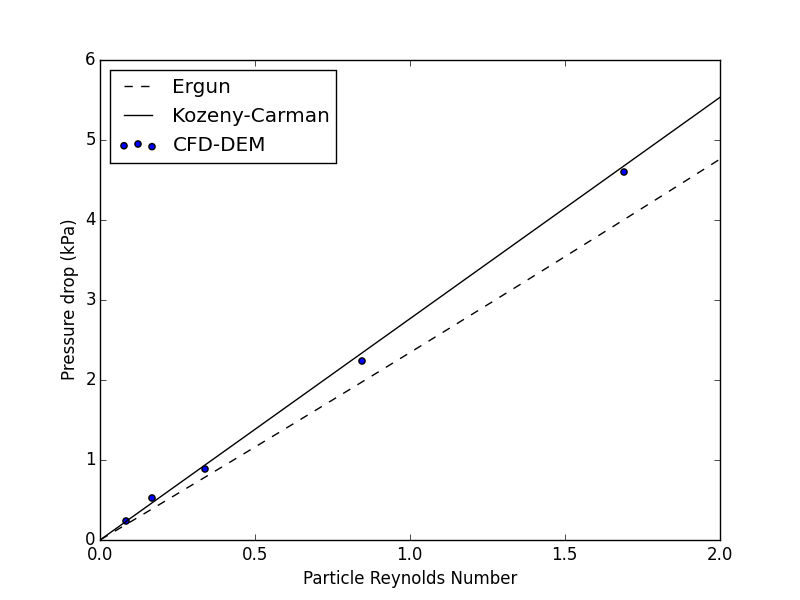
\includegraphics[width=\textwidth]{chapters/figures/pressureDrops-full.png}
                \caption{Well-packed bed}
                \label{fig:pressure-drop-full}
        \end{subfigure}%
        
          %add desired spacing between images, e. g. ~, \quad, \qquad, \hfill etc.
          %(or a blank line to force the subfigure onto a new line)
        \begin{subfigure}[b]{0.7\textwidth}
                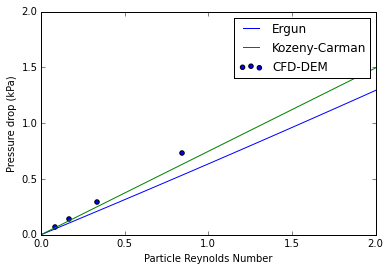
\includegraphics[width=\textwidth]{chapters/figures/pressureDrops-evap.png}
                \caption{Re-settled bed}
                \label{fig:pressure-drop-evap}
        \end{subfigure}
        \caption{Pressure drop calculations across packed beds, solved by CFD-DEM, fit well to the Kozeny-Carman empirical relation.}\label{fig:cfdem-pressure-drop}
\end{figure}